\appendix 

\section{Additional examples.}
\label{sec:app:examples}

\begin{figure*}
\centering
\begin{subfigure}{3in}
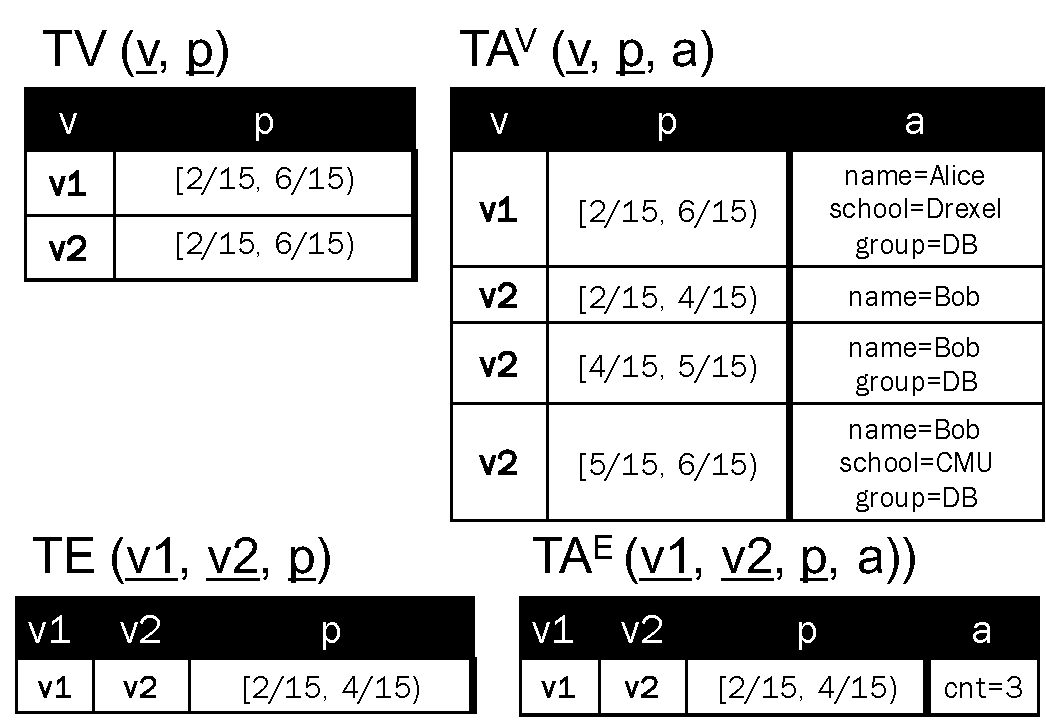
\includegraphics[width=2.8in]{figs/T1_inter_T2_rel.pdf}
\caption{$T1 \cap^T T2$.}
\vspace{-0.2cm}
\label{fig:tg_inter}
\end{subfigure}
\begin{subfigure}{3in}
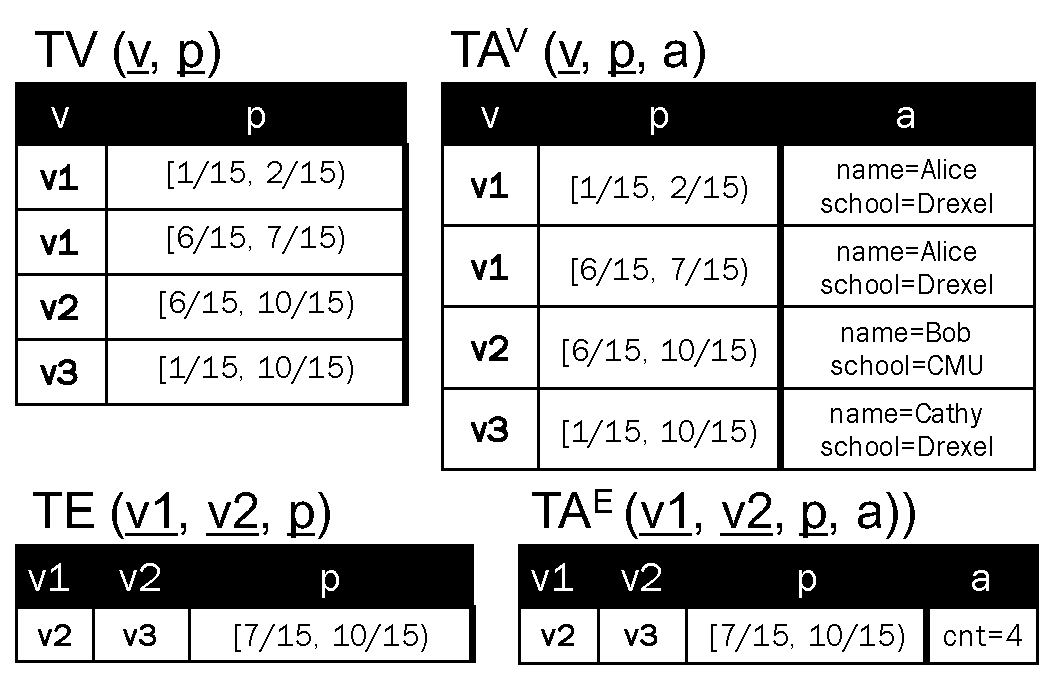
\includegraphics[width=2.8in]{figs/T1_diff_T2_rel.pdf}
\caption{$T1 \setminus^T T2$.}
\vspace{-0.2cm}
\label{fig:tg_diff}
\end{subfigure}
\caption{Binary operators.}
\label{fig:binary}
\vspace{-0.2cm}
\end{figure*}

Figure~\ref{fig:tg_inter} shows the result of temporal intersection
of \insql{T1} with \insql{T2}.  Only the vertices and edges present in
both \tgs are produced, thus eliminating $v_3$ and $v_4$.  Period
$[2/15, 4/15)$ for $v_2$ is computed as a result of the join of
$[2/15, 5/15)$ in \insql{T1} and [$2/15, 4/15)$ in \insql{T2}.

Figure~\ref{fig:tg_diff} shows the result of temporal difference
of \insql{T1} with \insql{T2}.  Vertex v1 is removed between 2/15 and
6/15, splitting one v1 tuple in \tv of T1 into two temporally-disjoint
tuples in the result.

\section{Additional results.}
\label{sec:app2}

Plots and discussion in this section complement experimental results
presented in Section~\ref{sec:exp}.

\begin{figure*}[th]
\centering
\begin{minipage}{2.1in}
\centering
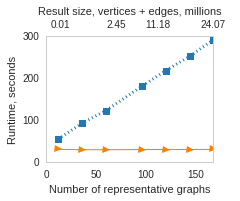
\includegraphics[width=2.1in]{figs/slice_wikitalk_build13.png}
\vspace{-0.2in}
\caption{Slice on wiki-talk.}
\label{fig:slicewiki}
\vspace{-0.1in}
\end{minipage}
\begin{minipage}{2.2in}
\centering
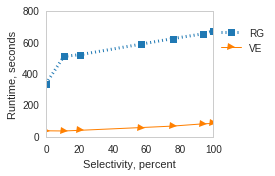
\includegraphics[width=2.2in]{figs/subgraph_wikitalk_build13.png}
\caption{Subgraph on wiki-talk.}
\vspace{-0.1in}
\label{fig:subgraphwiki}
\vspace{-0.1in}
\end{minipage}
\end{figure*}

